\documentclass[border=4pt]{standalone}
\usepackage{tikz}
\usetikzlibrary{arrows.meta,decorations.pathreplacing,backgrounds}

\begin{document}
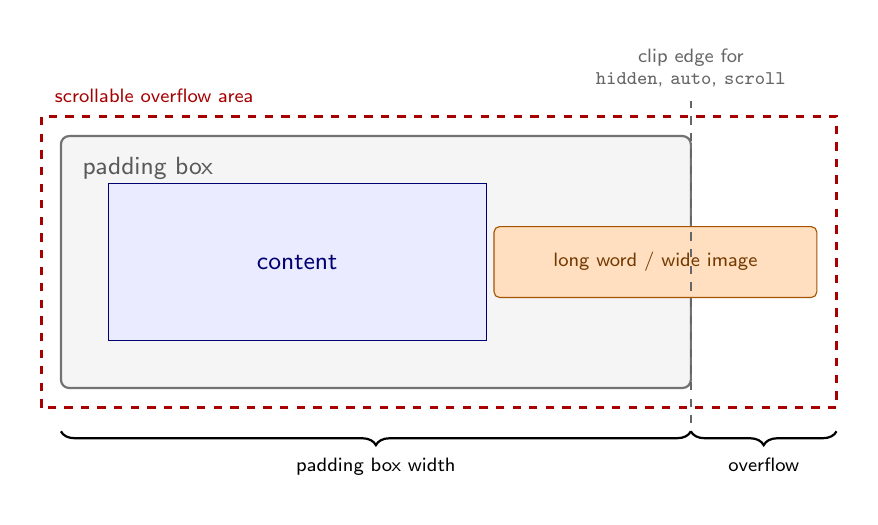
\begin{tikzpicture}[
  font=\sffamily\small,
  show background rectangle,
  background rectangle/.style={fill=white},
  brace/.style={decorate, decoration={brace, amplitude=5pt, mirror}, thick}
]
  % padding box
  \draw[thick, rounded corners=3pt, fill=gray!8, draw=black!55]
    (0,0) rectangle (8,3.2);
  \node[anchor=north west, text=black!65] at (0.15,3.05) {padding box};

  % content box
  \draw[fill=blue!8, draw=blue!45!black]
    (0.6,0.6) rectangle (5.4,2.6);
  \node[text=blue!45!black] at (3.0,1.6) {content};

  % overflowing element
  \draw[fill=orange!25, draw=orange!65!black, rounded corners=2pt]
    (5.5,1.15) rectangle (9.6,2.05);
  \node[text=orange!45!black, font=\sffamily\scriptsize]
    at (7.55,1.6) {long word / wide image};

  % scrollable overflow area
  \draw[dashed, very thick, red!65!black]
    (-0.25,-0.25) rectangle (9.85,3.45);
  \node[anchor=south west, text=red!65!black, font=\sffamily\scriptsize]
    at (-0.2,3.5) {scrollable overflow area};

  % clip edge
  \draw[dashed, thick, black!60] (8,-0.45) -- (8,3.65);
  \node[anchor=south, text=black!60, align=center, font=\sffamily\scriptsize]
    at (8,3.7) {clip edge for\\\texttt{hidden}, \texttt{auto}, \texttt{scroll}};

  % braces
  \draw[brace] (0,-0.55) -- (8,-0.55)
    node[midway, below=6pt, font=\sffamily\scriptsize] {padding box width};
  \draw[brace] (8,-0.55) -- (9.85,-0.55)
    node[midway, below=6pt, font=\sffamily\scriptsize] {overflow};
\end{tikzpicture}
\end{document}
